\documentclass{article}
\usepackage{array}
\usepackage[a4paper, total={6in, 8in}]{geometry}
\usepackage{graphicx}
\newcolumntype{L}[1]{>{\raggedright\let\newline\\\arraybackslash\hspace{0pt}}m{#1}}
\newcolumntype{C}[1]{>{\centering\let\newline\\\arraybackslash\hspace{0pt}}m{#1}}

\begin{document}
{\huge\textbf {1-System Level Structural Diagram}}
\\
\includegraphics[scale=0.8]{System_Level_Structural_Diagram}
\pagebreak
{\huge\textbf {2-Task Decomposition Graph}}
\\
{\huge {Module: Lap Counter}}
\\
\includegraphics[scale=0.2]{Lap_Counter_Task_Decomposition_Graph}
\\[0.2in]
{\huge {Module: Getting Speed Data from Input Device}}
\\[0.2in]
\includegraphics[scale=0.2]{Speed_Task_Decomposition_Graph}
\clearpage
{\huge\textbf {3-Sequence Diagram}}
\\
{\huge {Module: Lap Counter}}
\\
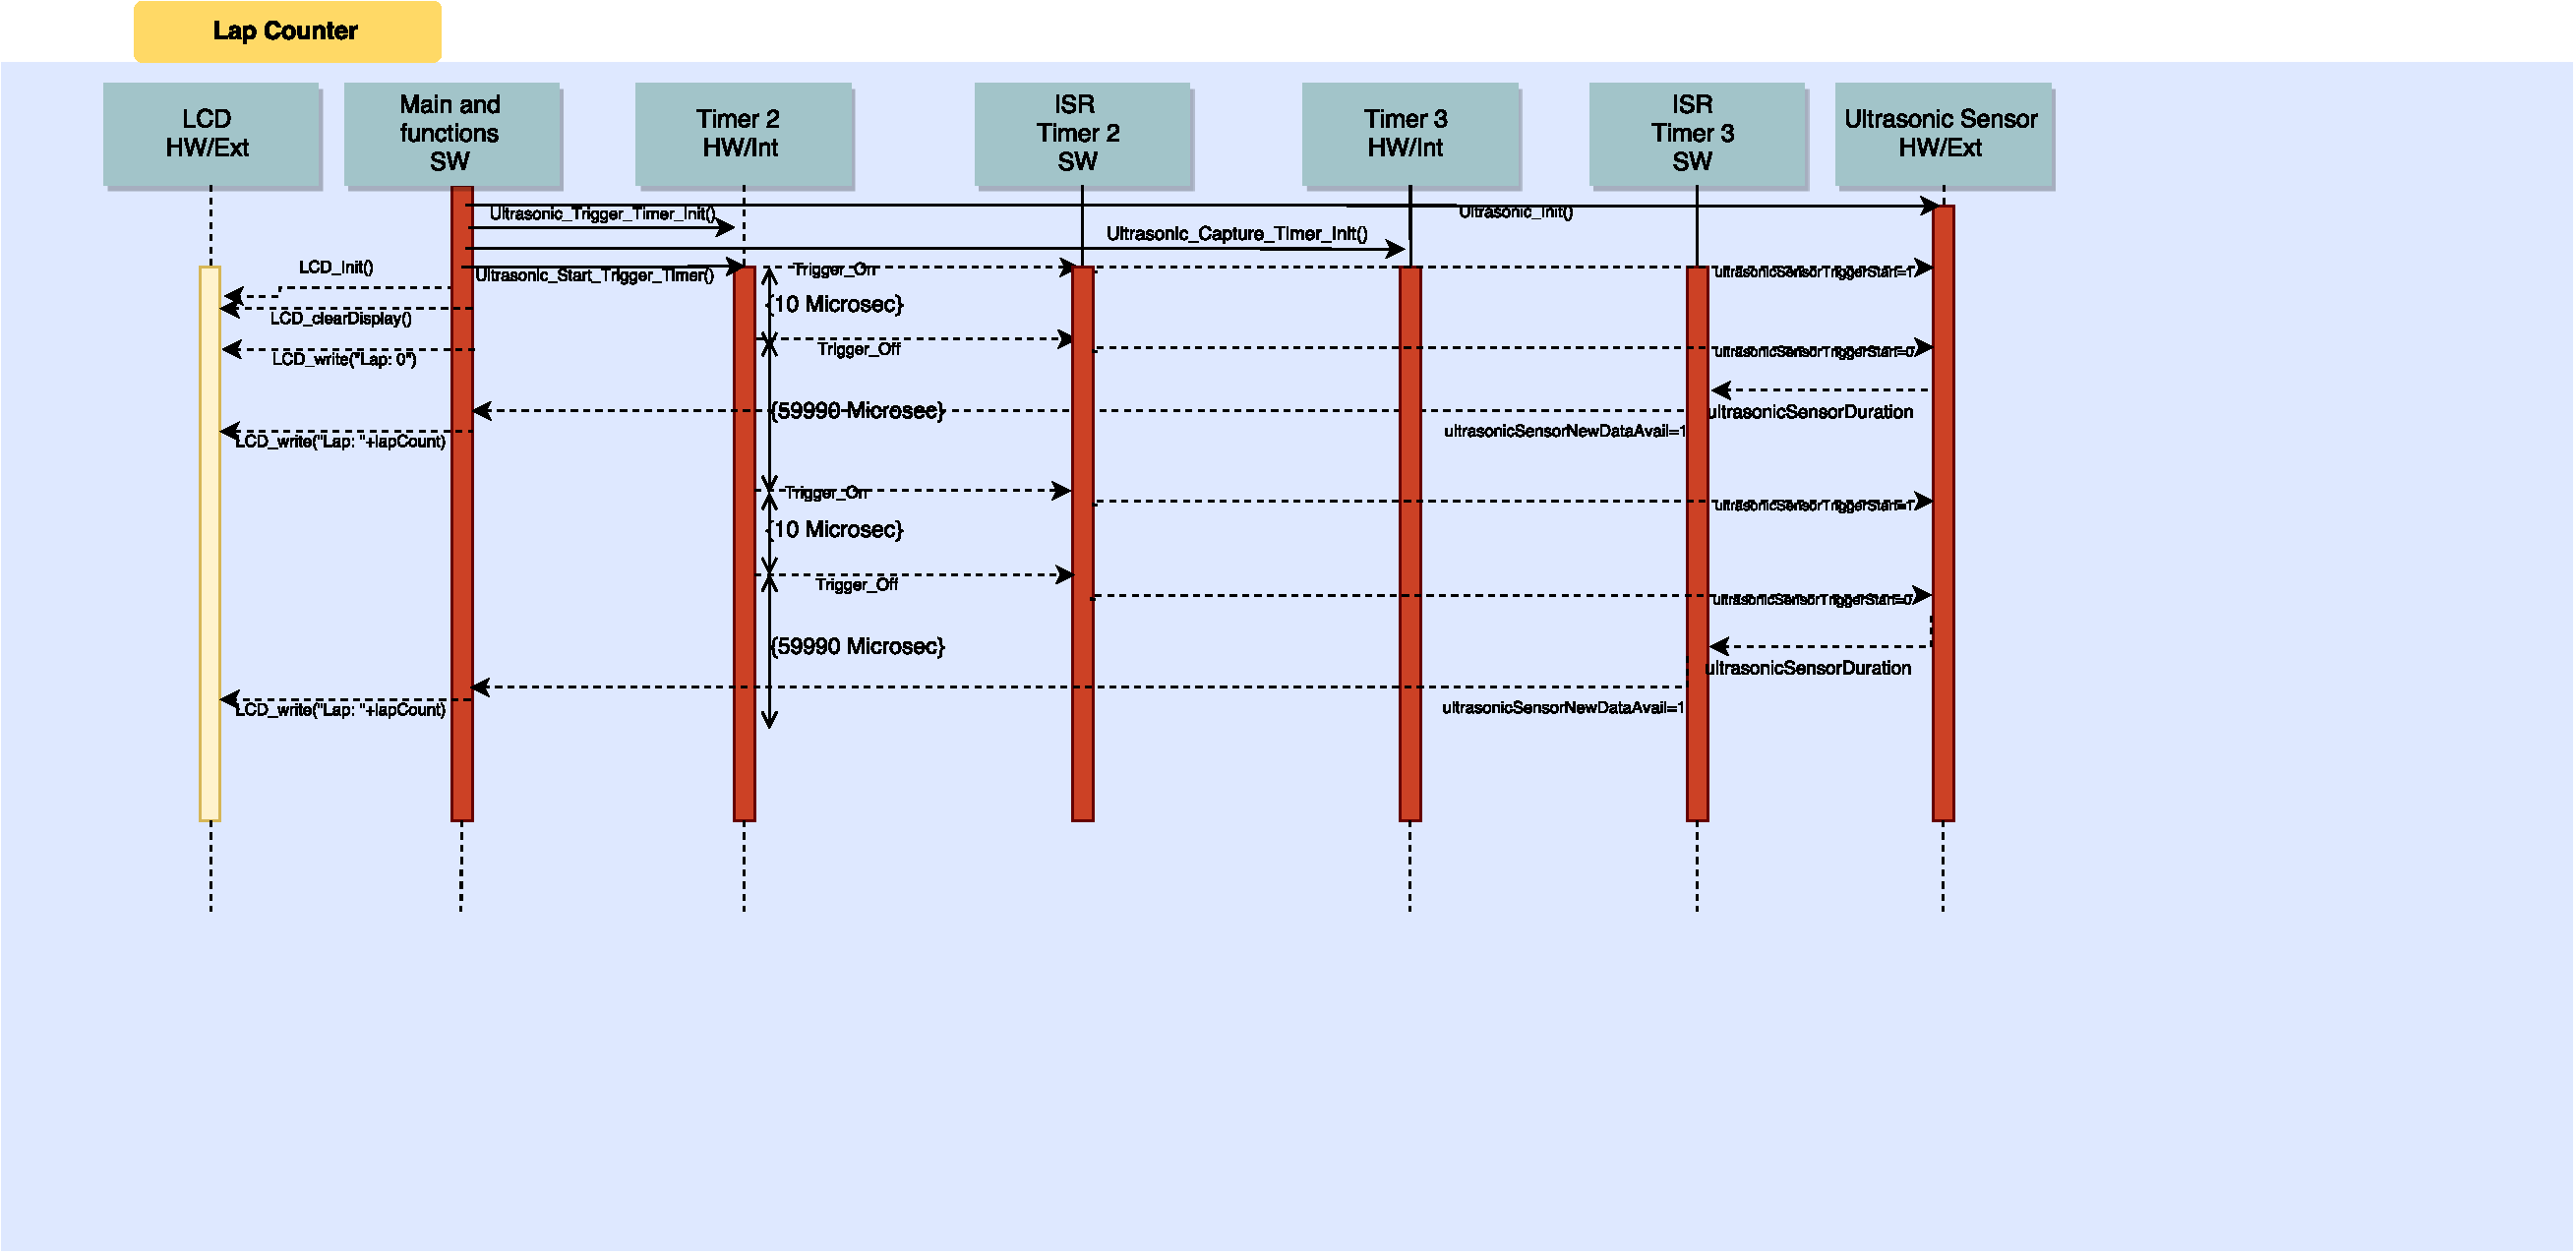
\includegraphics[scale=0.3]{Lap_Counter_Seq_Diagram}
\\
{\huge {Module: Getting Speed Data from Input Device}}
\\
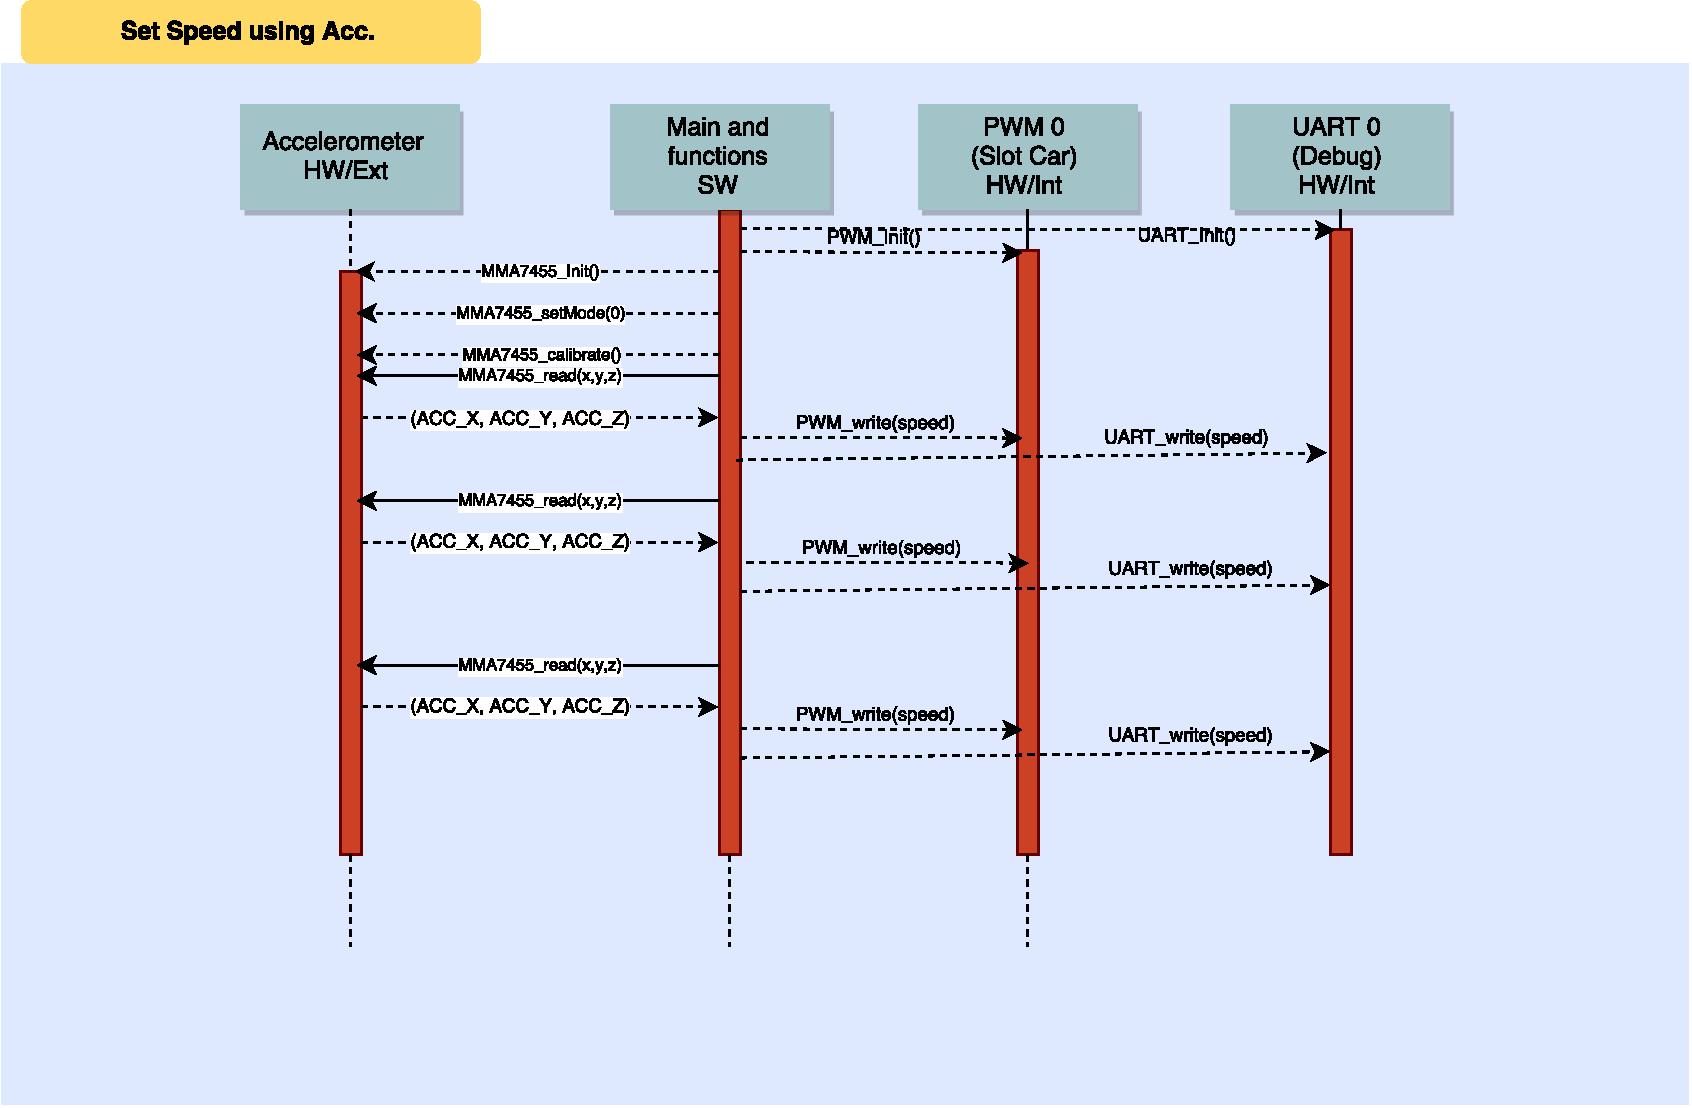
\includegraphics[scale=0.5]{Read_Acc_Control_Speed}
\clearpage
{\huge\textbf {4-Coding}}
\\
{\huge {Module: Lap Counter}}
\\
\begin{tabular}{| C{4cm} | C{4cm} | C{4cm} | C{2cm} |}
\hline
\textbf{Function Name} &\textbf{Function Definition}  & \textbf{Objective} &\textbf{WCET}\linebreak(simulation)\\
\hline
Ultrasonic\_Init() & Initialization of the Ultrasonic sensor. Functions of the trigger
and echo pins connected to the LPC board are defined in the IOCON registers& There are 2 data pins to
communicate with the ultrasonic sensor. Enabling the corresponding pins in the main board, their directions'
(input or output) is set for echo and trigger pins. So that, the board is able to trigger a calculation
of the distance and get the incoming signals with echo pin.& 18 usec\\
\hline
Ultrasonic\_Trigger\_Timer\_Init()&Trigger timer initializer. The output for the trigger pin is
 initialized in this function & Timer 2 is used to synchronize the value(either HIGH or LOW) to the Ultrasonic
 sensor. To initialized it, this function is used. First the power is enabled to this section with PCONP Register
 , then counters (Timer counters and Prescale counters) and match values are set appropriately. Last, the
 function on a match("toggle" in this case) is set. & 31 usec\\
\hline
LCD\_init()&Initialization of the LCD and its pins.& LCD is initialized by setting its pins' functionalities on the board,
and sending correct values to initialize the external driver, ( like 0x03, 0x03,0x03,0x02)&5.18 sec\\
\hline
\end{tabular}
\begin{tabular}{| C{4cm} | C{4cm} | C{4cm} | C{2cm} |}
\hline
Ultrasonic\_Capture\_Timer\_Init()& Echo timer initializer for the echo signal of the ultrasonic sensor.&
First the using PCONP register, the timer is powered on. Then its match registers and timer and prescale timer registers
are given the appropriate functionalities. This timer is used to count the elapsed time from the transmission of the
signals to the echo of the sent signals. So that, the distance of the object could be detected.&21.3 usec\\
\hline
Serial\_init()&Initialization of the UART 0 & Using UART(Serial communication), the debug information of distance of the detected object
and the lap count will be sent to the computer. &57.8 usec\\
\hline
TU()&Task for Ultrasonic, calculates the distance&The distance is calculated detected by ultrasonic sensor.
This distance is used to detect whether the car is in the range or not.&30.6 microsec\\
\hline
TC()& Task for the lap counter & After getting the distance detected, this function checks whether the
distance is smaller than the threshold, if it is, then the lap count is incremented by one. &23.0 microsec\\
\hline
TSD()&Task for system diagnosis, includes sending distance detected and the lap count data from UART
to PC & In order to debug the code, we are using this function which will be printing the value of
distance measured and the lap counted.&192 millisec\\
\hline
TDi()&This function sets the cursor to the appropriate position, then clears the display starting from the
cursor, then writes the lap count into the LCD screen.& To meet the requirements specified,
this function is used. It basically, writes the lap count into the LCD screen.&12.2 microsec\\
\hline
\end{tabular}
{\huge {Module: Getting Speed Data from Input Device}}
\\
\begin{tabular}{| C{4cm} | C{4cm} | C{4cm} | C{2cm} |}
\hline
\textbf{Function Name} &\textbf{Function Definition}  & \textbf{Objective} &\textbf{WCET}\linebreak(simulation)\\
\hline
TI()&Function initializes all the devices/modules used by the operating code.Basically consists of initializing
accelerometer, PWM pin, &In order to use the devices in the board, we have to initialize them before using.
Powering on the devices(PCONP) and giving the appropriate pin functionalities(IOCON) are done in this step.&5.86 secs\\
\hline
TSS()&Task for setting the speed of the car. To set a speed, first we are reading the angle of the board, from the
accelerometer. Using the angle value of it, the pulse width of the output signal is modulated from 0 to 999 where 500
means that 50\% duty cycle.& To meet the requirements specified, we are using the accelerometer data as input to
set the speed of the slot car. After getting the angle value, the speed of the car is set by using PWM.&44.6 microsec\\
\hline
TGA()&Task for getting the angle of the board using the accelerometer device on it. This function reads the
acceleration data from the device on the LPC board and finds the angle in the X dimension of the device.&
To make the speed of the slot car controllable by an input device, accelerometer device is used and according to
its angle in the X direction, the speed of the car is set. This function realizes the getting the angle data.&79.7 microsec\\
\hline
TSD()&Task for system diagnosis. This function is used to send the speed information to the PC using UART.&To debug the
code that we wrote in this section, the data produced is sent to the PC to oversee the system working.&522 millisec\\
\hline
\end{tabular}
\clearpage
{\huge\textbf {5-Scheduling}}
\\
{\huge {Module: Lap Counter}}
\\
{\huge {Module: Getting Speed Data from Input Device}}
\clearpage
{\huge\textbf {6-Timing Diagram}}
\\
{\huge {Module: Lap Counter}}
\\
{\huge {Module: Getting Speed Data from Input Device}}
\clearpage
{\huge\textbf {7-Hardware Block Diagram}}
\\
{\huge {Module: Lap Counter}}
\\
{\huge {Module: Getting Speed Data from Input Device}}
\clearpage
{\huge\textbf {8-Board Pin Table}}
\\
{\huge {Module: Lap Counter}}
\\
{\huge {Module: Getting Speed Data from Input Device}}
\\
\end{document}
